\documentclass[xcolor=dvipsnames,table]{beamer}

\usepackage{latexsym}
\usepackage[utf8]{inputenc}
\usepackage[brazil]{babel}
\usepackage{amssymb}
\usepackage{amsmath}
\usepackage{stmaryrd}
\usepackage{fancybox}
\usepackage{datetime}
\usepackage[T1]{fontenc}
\usepackage{graphicx}
\usepackage{graphics}
\usepackage{url}
\usepackage{algorithmic}
\usepackage{algorithm}
\usepackage{acronym}
\usepackage{array}

\newtheorem{definicao}{Definio}
\newcommand{\tab}{\hspace*{2em}}

\mode<presentation>
{
  \definecolor{colortexto}{RGB}{0,0,0}
 
  \setbeamertemplate{background canvas}[vertical shading][ bottom=white!10,top=white!10]
  \setbeamercolor{normal text}{fg=colortexto} 

  \usetheme{Warsaw}
}

\title{Complexidade de Tempo} 

\author{
  Esdras Lins Bispo Jr. \\ \url{bispojr@ufg.br}
  } 
 \institute{
  Teoria da Computação \\Bacharelado em Ciência da Computação}
\date{\textbf{07 de agosto de 2017} }

\logo{
\includegraphics[width=1cm]{images/ufgJataiLogo.png}}

\begin{document}

	\begin{frame}
		\titlepage
	\end{frame}

	\AtBeginSection{
		\begin{frame}{Sumário}%[allowframebreaks]{Sumário}
    		\tableofcontents[currentsection]
    		%\tableofcontents[currentsection, hideothersubsections]
		\end{frame}
	}

	\begin{frame}{Plano de Aula}
		\tableofcontents
		%\tableofcontents[hideallsubsections]
	\end{frame}
    
    \section{Revisão}
	
	\subsection{Problema da Parada}
	\begin{frame}{Problema da Parada}
		\begin{block}{$A_{MT}$ é indecidível (Ideia da prova)}
			\begin{itemize}
				\item Vamos supor que $H$ decida $A_{MT}$   
				\item Vamos construir a MT $D$ conforme a descrição abaixo:\\   
				$D$ = ``Sobre a entrada $\langle M \rangle$, em que $M$ é uma MT:
				\begin{enumerate}
					\item Rode $H$ sobre a entrada $\langle M, \langle M \rangle \rangle$.
					\item Dê como saída o oposto do que $H$ dá como saída; ou seja, se $H$ aceita, {\it rejeite} e se $H$ rejeita, {\it aceite}.''
				\end{enumerate}   
				\item Entretanto, $D(\langle D \rangle)$ leva a uma contradição.   
				\item Logo, $A_{MT}$ é indecidível.
			\end{itemize}
		\end{block}
	\end{frame}

	\begin{frame}{Problema da Parada}
		\begin{block}{$A_{MT}$ é indecidível (Ideia da prova)}
			Resumindo...   
			\begin{itemize}
				\item $H$ aceita $\langle M, \omega \rangle$ exatamente quando $M$ aceita $\omega$.   
				\item $D$ rejeita $\langle M \rangle$ exatamente quando $M$ aceita $\langle M \rangle$.   
				\item $D$ rejeita $\langle D \rangle$ exatamente quando $D$ aceita $\langle D \rangle$ ({\color{red} Absurdo!!!}).
			\end{itemize}
		\end{block}
	\end{frame}

	\begin{frame}{Problema da Parada}
		\begin{center}
			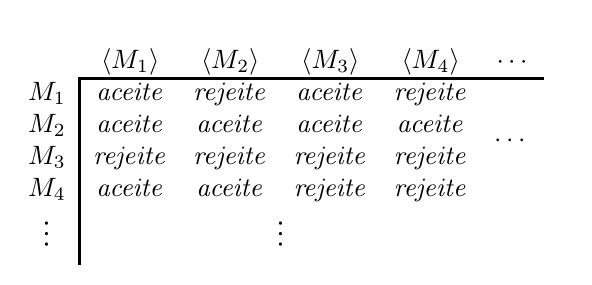
\includegraphics[width=11cm]{images/h.png}
			
			 A entrada $i,j$ é o valor de $H$ sobre a entrada $\langle M_i , \langle M_j \rangle \rangle$.
		\end{center}
	\end{frame}

	\begin{frame}{Problema da Parada}
		\begin{center}
			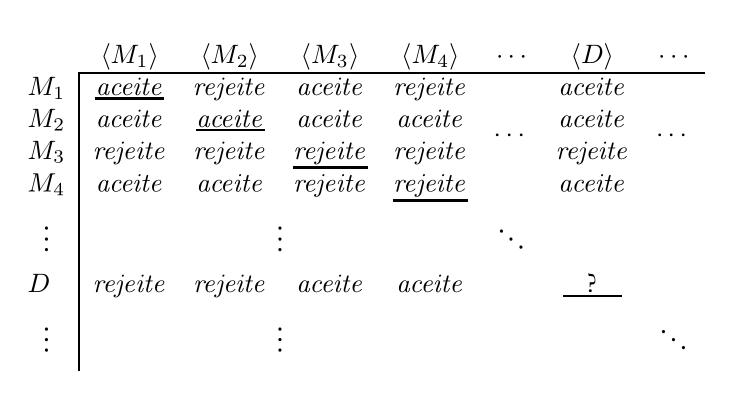
\includegraphics[width=11cm]{images/d.png}
			
			{\bf Figura:} Se D estiver na figura, uma contradição ocorre em ``?''.
		\end{center}
	\end{frame}

	\subsection{Linguagem Turing-Irreconhecíveis}
	\begin{frame}{Linguagens Turing-irreconhecíveis}
		\begin{block}{Teorema 4.22}
			Uma linguagem é decidível sse ela é Turing-reconhecível e co-Turing-reconhecível.
		\end{block}   
		\begin{block}{Corolário 4.23}
			$\overline{A_{MT}}$ não é Turing-reconhecível.
		\end{block}
	\end{frame}

		\section{Complexidade de Tempo}	
	\begin{frame}{Complexidade}
		\begin{block}{Por que estudar complexidade?}
			Um problema pode ser até decidível, mas pode levar uma quantidade de tempo ou memória bastante elevada.
		\end{block} \pause
		\begin{block}{Questões do estudo de complexidade}
			\begin{itemize}
				\item Quanto tempo[espaço] leva[ocupa] um determinado algoritmo?
				\item O que faz um algoritmo gastar[ocupar] mais tempo[espaço] do que um outro?
				\item É possível classificar os algoritmos em termos de complexidade?
			\end{itemize}
		\end{block}
	\end{frame}
	
	\begin{frame}[shrink]{Complexidade de Tempo}
		\begin{block}{Problema}
			Seja a linguagem $A = \{ 0^k 1^k$ | $k \geq 0 \}$. Quanto tempo uma máquina de Turing simples precisa para decidir $A$?
		\end{block} \pause
		\begin{block}{Descrição de uma possível MT simples}
			$M_1$ = ``Sobre a cadeia de entrada $\omega$:
			\begin{enumerate}
				\item Faça uma varredura na fita e {\it rejeite} se um 0 for encontrado à direita de um 1.
				\item Repita se ambos 0s e 1s permanecem sobre a fita:
				\begin{enumerate}
					\item Faça uma varredura na fita, cortando um único 0 e um único 1.
				\end{enumerate}
				\item Se 0s ainda permanecerem após todos os 1s tiverem sido cortados, ou se 1s ainda permanecerem após todos os 0s tiverem sido cortados, {\it rejeite}. Caso contrário, se nem 0s nem 1s permanecerem sobre a fita, {\it aceite}.
			\end{enumerate}
		\end{block}
	\end{frame}
	
	\begin{frame}{Complexidade de Tempo}
		\begin{block}{Analisando a entrada}
			\begin{itemize}
				\item Grafo: número de nós, número de arestas;
				\item Estrutura de dados: tamanho do vetor, altura da árvore;
				\item Cadeia: tamanho da cadeia de entrada.
			\end{itemize}
		\end{block} \pause
		\begin{block}{Tipos de Análise}
			\begin{itemize}
				\item Análise do pior caso;
				\item Análise do caso médio;
				\item Análise do melhor caso.
			\end{itemize}
		\end{block} \pause
		\begin{block}{Utilizaremos aqui...}
			O tamanho da cadeia de entrada e a análise de pior caso.
		\end{block}
	\end{frame}
	
	\begin{frame}{Complexidade de Tempo}
		\begin{block}{Definição 7.1}
			Seja $M$ uma máquina de Turing determinística que pára sobre todas as entradas. O tempo de execução ou {\bf complexidade de tempo} de $M$ é a função $f : \mathbb{N} \rightarrow \mathbb{N}$, em que $f(n)$ é o número máximo de passos
			que $M$ usa sobre qualquer entrada de comprimento $n$.
			
			\vspace*{0.3cm}
			
			Se $f(n)$ for o tempo de execução de $M$, dizemos que $M$ {\it roda} em tempo $f(n)$ e que $M$ é uma máquina de Turing {\it de tempo} $f(n)$. Costumeiramente usamos $n$ para representar o comprimento da entrada.
		\end{block}
	\end{frame}
	
	\begin{frame}{Complexidade de Tempo}
		\begin{block}{Notação O-Grande}
			Sejam $f$ e $g$ funções $f,g:\mathbb{N} \rightarrow \mathbb{R}^+$ . \\Vamos dizer que $f(n) = O(g(n))$ se inteiros positivos $c$ e $n_0$ existem tais que para todo inteiro $n \geq n_0$ em que
			\begin{center}
				$f(n) \leq c.g(n)$			
			\end{center}
			Quando $f(n) = O(g(n))$, dizemos que $g(n)$ é um {\bf limitante superior} para $f(n)$, ou mais precisamente, que $g(n)$ é um {\bf limitante superior assintótico} para $f(n)$, para enfatizar que estamos suprimindo fatores constantes.
		\end{block}
	\end{frame}
	
	\begin{frame}{Complexidade de Tempo}
		\begin{center}
			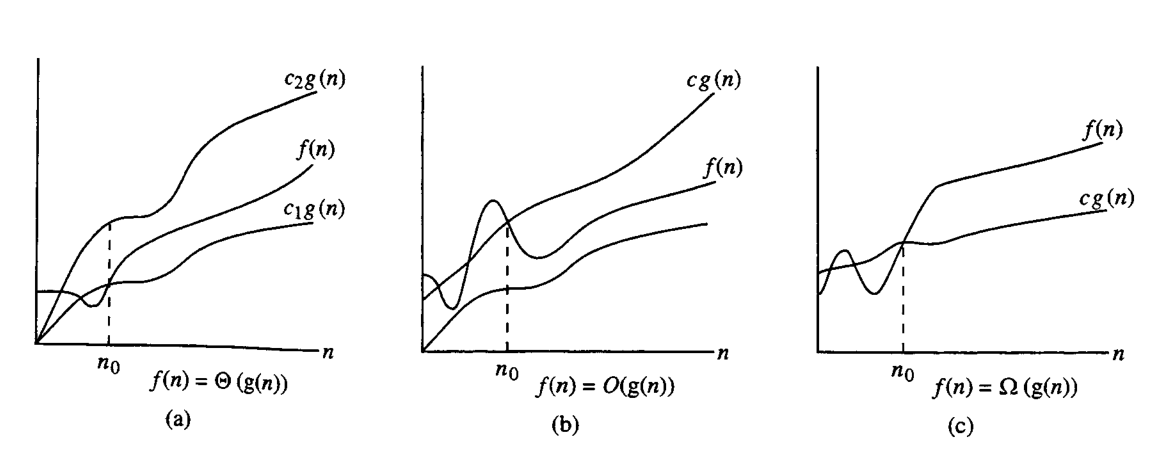
\includegraphics[width=11cm]{images/crescimento.png}
			
			{\bf Figura:} Comportamento das notações $\Theta$, $O$ e $\Omega$.
		\end{center}
	\end{frame}	
	
	\begin{frame}{Complexidade de Tempo}
		\begin{block}{$f_1 (n) = 5n^3 + 2n^2 + 22n + 6$}
			\begin{eqnarray}
			O(f_1(n)) & = & O(5n^3 + 2n^2 + 22n + 6)\\
			& = & O(5n^3)\\
			& = & O(n^3)
			\end{eqnarray}
		\end{block} \pause
		\begin{exampleblock}{É verdade porque...}
			Basta admitir $c = 6$, e $n_0 = 10$. Logo
			\begin{center}
				$5n^3 + 2n^2 + 22n + 6 \leq 6n^3$
			\end{center}
			para todo $n \geq 10$.
		\end{exampleblock}
	\end{frame}
	
	\begin{frame}{Complexidade de Tempo}
		\begin{block}{$f_1 (n) = 5n^3 + 2n^2 + 22n + 6$}
			\begin{eqnarray}
			O(f_1(n)) & = & O(5n^3 + 2n^2 + 22n + 6)\\
			& = & O(5n^3)\\
			& = & O(n^3)
			\end{eqnarray}
		\end{block} \pause
		\begin{exampleblock}{Também é verdade dizer que...}
			$f_1(n) = O(n^4)$, pois $n^4$ é maior que $n^3$ e portanto é ainda um limitante assintótico superior sobre $f_1$.
		\end{exampleblock} \pause
		\begin{alertblock}{Mas...}
			$f_1(n) \not= O(n^2)$.
		\end{alertblock}
	\end{frame}
	
	\begin{frame}{Complexidade de Tempo}
		\begin{block}{$f_2 (n) = \mbox{log}_{13} n + 5$}
			\begin{eqnarray} \pause
			O(f_2(n)) & = & O(\mbox{log}_{13} n + 5)\\
			& = & O(\mbox{log}_{13} n)\\
			& = & O(\mbox{log} n)
			\end{eqnarray}
		\end{block} \pause
		\begin{exampleblock}{Porque...}
			$\mbox{log} n = \mbox{log}_{10} n  = \frac{\mbox{log}_{13} n}{\mbox{log}_{13} 10}$
		\end{exampleblock}
	\end{frame}
	
	\begin{frame}{Complexidade de Tempo}
		\begin{block}{$f_3 (n) =  3n \mbox{log}_2 n + 5n \mbox{log}_2 \mbox{log}_2 n + 2$}
			\begin{eqnarray} \pause
			O(f_3(n)) & = & O(3n \mbox{log}_2 n + 5n \mbox{log}_2 \mbox{log}_2 n + 2)\\
			& = & O(3n \mbox{log}_2 n)\\
			& = & O(n \mbox{log} n)
			\end{eqnarray}
		\end{block} \pause
		\begin{exampleblock}{Porque...}
			$\mbox{log} n$ domina sobre $\mbox{log} \mbox{log} n$.
		\end{exampleblock}
	\end{frame}
	
	\begin{frame}
		\titlepage
	\end{frame}
	
\end{document}